\chapter{A chapter}
\label{cha:a_chapter}

This is the first paragraph of the \PolyTeXnic\ template. For more information, see \emph{The \PolyTeXnic\ Book}}, available online at \href{http://polytexnic.org/book}{http://polytexnic.org/book}.

This is the \emph{second} paragraph, showing how to emphasize text.\footnote{\emph{This} is a footnote. It is numbered automatically.} You can also make text \textbf{bold} or \textit{italicized} (which looks the same as emphasized text).

\section{A section}
\label{sec:a_section}

This is a section. Because it has a label, we can refer to it as Section~\ref{sec:a_section}; the cross-reference will be automatically numbered and linked.

\subsection{Source code}
\label{sec:source_code}

This is a subsection. As usual, it can be referenced by label (Section~\ref{sec:source_code}). Note that the label starts with \texttt{sec:}, not \texttt{ssec:} or \texttt{subsec:}. Any of these would work, but I find that sections often become subsections (and vice versa) when figuring out the structure of a book, and using \texttt{sec:} to prefix them both saves having to change the labels.

\PolyTeXnic\ comes with full support for syntax-highlighted source code:
%= lang:ruby
\begin{code}
def hello
  puts "hello, world!"
end
\end{code}
\PolyTeXnic\ can highlight any language supported by \href{http://pygments.org/languages/}{Pygments}.

You can also define code \emph{listings}, as seen in Listing~\ref{code:hello_world}. Such code listings are automatically numbered and linked.

\begin{codelisting}
\label{code:hello_world}
\codecaption{``Hello, world!'' in Ruby.}
%= lang:ruby
\begin{code}
def hello
  puts "hello, world!"
end
\end{code}
\end{codelisting}

You can also typeset inline code, as in \kode{current\_\-user}. If you prefer a plainer version of the same thing, you can use ``typewriter text'', as in \texttt{current\_\-user}.

For words whose hypenation isn't built in, you can indicate an optional hyphen using \verb+\-+, which will only be used if necessary to make a clean line break (and even then only when producing PDFs):
%= lang:latex
\begin{code}
current\_\-user
\end{code}
This also shows how to escape the underscore character using a backslash. This is because plain underscores are reserved for math environments (Section~\ref{sec:mathematics}).

\subsection{Mathematics}
\label{sec:mathematics}

\PolyTeXnic\ supports full mathematical typesetting, including inline math, such as $\phi^2 - \phi - 1 = 0$, and centered math, such as
\[ \phi = \frac{1+\sqrt{5}}{2}. \]
It also support cross-referenced equations, as in Eq.~\eqref{eq:golden_ratio} and Eq.~\eqref{eq:stokes_theorem}.

\begin{equation}
\label{eq:golden_ratio}
\phi = \frac{1+\sqrt{5}}{2} \approx 1.618 \qquad{\text{The Golden Ratio}}
\end{equation}

\begin{equation}
\label{eq:stokes_theorem}
\int_\Omega d\omega = \int_{\partial\Omega} \omega \qquad{\text{Stokes's Theorem}}
\end{equation}

\PolyTeXnic\

Include graphics like this:

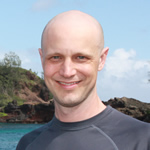
\includegraphics{images/2011_michael_hartl.png}

\image{images/2011_michael_hartl.png}

Include code like this:

%= lang:ruby
\begin{code}
def hello
  "hello, world!"
end
\end{code}

Make a code listing as in Listing~\ref{code:hello}.

\begin{codelisting}
\label{code:hello}
\codecaption{A hello program in Ruby.}
%= lang:ruby
\begin{code}
def hello
  "hello, world!"
end
\end{code}
\end{codelisting}

Typeset inline code using the \verb+\kode+ environment: \kode{foobar}.

\section{\emph{Bacon} ipsum}
\label{sec:bacon_ipsum}

\begin{table}
\begin{tabular}{llll}
\textbf{HTTP request} & \textbf{URL} & \textbf{Action} & \textbf{Purpose} \\ \hline

\texttt{GET} & /users & \texttt{index} & page to list all users \\
\texttt{GET} & /users/1 & \texttt{show} & page to show user with id \texttt{1}\\
\texttt{GET} & /users/new & \texttt{new} & page to make a new user \\
\texttt{POST} & /users & \texttt{create} & create a new user \\
\texttt{GET} & /users/1/edit & \texttt{edit} & page to edit user with id \texttt{1} \\
\texttt{PATCH} & /users/1 & \texttt{update} & update user with id \texttt{1}  \\
\texttt{DELETE} & /users/1 & \texttt{destroy} & delete user with id \texttt{1}
\end{tabular}
\caption{HTTP stuff\label{table:foo}}
\end{table}


Bacon ipsum dolor sit amet salami doner shoulder, brisket pork chop beef cow bacon strip steak filet mignon jerky bresaola turducken venison ham. Biltong meatloaf chuck rump pork loin. Pancetta fatback prosciutto shankle corned beef flank beef ribs tail tri-tip kielbasa drumstick. Andouille bacon pork drumstick meatball pig t-bone hamburger, ball tip meatloaf sausage.

This is some math: $\int_a^b f'\,dx = f(b) - f(a)$.

See Chapter~\ref{cha:foo_bar} and Section~\ref{sec:pig_fatback}.

\subsection{Pig fatback}
\label{sec:pig_fatback}

Pig fatback beef ribs tongue ribeye bacon. Pig meatball salami, pastrami beef swine ham pork tail tongue shank bresaola turkey. Chuck cow shank short ribs pork belly short loin pastrami turkey. Pork loin doner tri-tip boudin brisket.
